%% =====================================================================
%%  Home Energy Coach -- Project Proposal
%%  High Integrity Systems, Winter Semester 2026/27
%%  Frankfurt University of Applied Sciences, Prof. Dr. Christina Andersson
%% ---------------------------------------------------------------------
%%  Compile with pdflatex (IEEEtran class, included in Overleaf / TeX Live).
%%  The diagrams are PNGs in figures/; edit the matching figures/*.tex
%%  source and run ./build-figures.sh to re-render them.
%%  Everything printed in RED is a placeholder:
%%     \ph{...}                 short placeholders (names, matriculation numbers, links)
%%     \begin{phsection}...     the whole section reserved for the ML / data-mining models
%%  Search the file for "\ph{" and "phsection" to find them all.
%% =====================================================================
\documentclass[conference]{IEEEtran}
\usepackage[utf8]{inputenc}
\usepackage[T1]{fontenc}
\usepackage{textcomp}
\usepackage{graphicx}
\usepackage{booktabs}
\usepackage{array}
\usepackage{xcolor}
\usepackage{url}
\usepackage[hidelinks]{hyperref}

% ---------- placeholders -------------------------------------------------
\newcommand{\ph}[1]{\textcolor{red}{\textbf{[#1]}}}
% A whole placeholder section: red rules above and below, dark-red text.
% (Breakable across columns, unlike a framed box.)
\newenvironment{phsection}[1]{%
  \par\noindent\textcolor{red}{\rule{\columnwidth}{0.8pt}}\par\smallskip
  \noindent\textbf{\textcolor{red}{PLACEHOLDER -- #1}}\par\smallskip
  \color{red!55!black}}{%
  \par\smallskip\noindent\textcolor{red}{\rule{\columnwidth}{0.8pt}}\par}
% ---------- small helpers ------------------------------------------------
\newcommand{\COtwo}{CO$_2$}
\newcommand{\pkg}[1]{\texttt{#1}}
\newcolumntype{L}[1]{>{\raggedright\arraybackslash}p{#1}}   % left-aligned, no justification gaps

\begin{document}

\title{Project Proposal: Home Energy Coach\\
{\large A Personalized Green Habit Recommender for Students and Renters in Shared Flats}}

\author{
  \IEEEauthorblockN{Muhammad Saad Zafar\textsuperscript{1541621},
    Asif Newaz\textsuperscript{matriculation no},
    Mazba Uddin\textsuperscript{matriculation no},\\
    Madhusudan Abhay Ambulkar Athar\textsuperscript{matriculation no},
    Nazmul Alam\textsuperscript{matriculation no},
    Md. Rabiul Hasan Tanvir\textsuperscript{matriculation no}}
\IEEEauthorblockA{Frankfurt University of Applied Sciences\\
High Integrity Systems -- Winter Semester 2026/27\\
Supervisor: Prof.\ Dr.\ Christina Andersson}
}

\maketitle

\begin{abstract}
This proposal outlines the design and development plan for \emph{Home Energy Coach}, a Personalized Green Habit Recommender developed as part of the High Integrity Systems Project at Frankfurt University of Applied Sciences (WS~2026/27). The application targets students and renters in shared flats (WGs), who cannot change their building's insulation or heating system but can change their daily habits. Users complete a short energy profile, receive a ranked feed of habits that fit their flat and schedule, commit to one small goal at a time and are prompted at the right moment. The signature feature is the \emph{Green Hours planner}: using live generation data of the German electricity market from the Bundesnetzagentur's SMARD platform, it tells each user the lowest-\COtwo{} hours for laundry, dishwasher and charging, fitted to the hours they are actually at home. A FastAPI back-end coordinates the application logic and delegates all data analysis -- the hourly \COtwo{} forecast, recommendation ranking, association-rule mining, user clustering and the evaluation of nudges -- to an R analytics service exposed through the \pkg{plumber} package. User data is persisted in PostgreSQL and the whole system is containerized with Docker. In line with the course's green software requirement, the energy and resource consumption of the application itself is measured from the first prototype on, reduced in every sprint and shown to users in the app. The project follows Scrum over five sprints with rotating Scrum Master and Product Owner roles, and all progress is tracked in Jira.
\end{abstract}

\section{Introduction}
Private households account for a substantial share of Germany's final energy consumption, and within a household more than two thirds of that energy goes into space heating, followed at a distance by hot water, cooking and electrical appliances~\cite{uba-haushalte}. Most of the advice households receive therefore targets the building: insulate, replace the boiler, install a heat pump. Students and other renters -- and in particular the residents of shared flats (Wohngemeinschaften, WGs) -- cannot act on any of it. They do not own the building, rarely choose the heating system or the electricity contract, and often never see their own consumption because the flat receives a single bill. What they \emph{can} change is their daily behaviour: how rooms are heated and ventilated, how long showers last, which devices stay on standby and, increasingly important, \emph{when} appliances run.

The timing aspect is what makes this project more than a list of tips. The \COtwo{} intensity of German electricity varies strongly within a day because the share of wind and solar generation changes from hour to hour. The Bundesnetzagentur publishes actual and forecast generation per energy source and the actual consumption for Germany on its SMARD platform, free of charge and in machine-readable form~\cite{smard}. From this data an hourly \COtwo{} intensity can be computed, and a washing-machine load, a dishwasher run or the charging of a laptop can be shifted into the cleanest hours -- provided the user is at home then. This is the idea behind the \emph{Green Hours planner}, the signature feature of Home Energy Coach.

Information alone, however, rarely changes behaviour; the gap between good intentions and action is well documented. Home Energy Coach is therefore designed as a habit-building system rather than an information app. It follows the Fogg Behavior Model, in which a behaviour occurs only when motivation, ability and a prompt come together at the same moment~\cite{fogg2009}, and the habit loop of cue, routine and reward. Users commit to one small, concrete goal at a time -- an implementation intention of the form ``when X, I do Y''~\cite{gollwitzer1999} -- are prompted exactly when the green window opens, and see the saved \COtwo{} and their streak immediately afterwards. Behaviour that is repeated in the same context for several weeks becomes automatic~\cite{lally2010}; the app then fades its prompts and proposes the next habit.

This proposal describes the planned development of Home Energy Coach as the team's realisation of the course topic \emph{Personalized Green Habit Recommender}. The system consists of a front-end (web or native iOS, see Section~\ref{sec:frontend}), a FastAPI back-end and an R analytics service that performs all data analysis and data mining tasks and is accessed through the \pkg{plumber} package. Development follows Scrum over five sprints, with all work tracked in Jira and source code managed collaboratively on GitHub. A particular advantage of the chosen domain is that the team itself belongs to the target group, so the app can be piloted on its own developers in the final sprint.

\subsection{Objectives}
\begin{enumerate}
\item Build a platform that recommends personalized home-energy habits to students and renters and prompts them at the right moment, including the greenest hours of the day derived from live German grid data.
\item Use R~\cite{rcore} for all data analysis and data mining tasks: the hourly \COtwo{} forecast, the recommendation ranking, association rules, clustering and the evaluation of nudges.
\item Deliver at least eight distinct user interfaces beyond standard CRUD and authentication screens; eleven are planned (Section~\ref{sec:ui}).
\item Measure the energy and resource consumption of the application itself from the first prototype on, and reduce it in every subsequent sprint.
\item Follow Scrum~\cite{scrumguide} with rotating Scrum Master and Product Owner roles, with all progress tracked in Jira.
\end{enumerate}

\subsection{Topic Selection}
The course fixes the topic but leaves the application domain open. The team shortlisted six candidate domains and scored them from 1 to 5 against five criteria derived from the course brief: availability of real data (weight 30\,\%), fit with a cue--routine--reward habit loop (25\,\%), number of meaningful screens (15\,\%), feasibility within one semester (15\,\%) and whether the team can test the app on itself (15\,\%). Table~\ref{tab:selection} shows the result. Home Energy Coach scored highest, mainly because of the free, high-resolution SMARD data and the natural habit loop around appliance timing. The campus-challenge idea survives as the WG and campus challenge feature inside the winner.

\begin{table}[!t]
\caption{Scoring of the Shortlisted Domains (1--5 per Criterion)}
\label{tab:selection}
\centering
\scriptsize
\setlength{\tabcolsep}{3.5pt}
\begin{tabular}{@{}lcccccc@{}}
\toprule
Candidate & Real data & Habit loop & Screens & Doable & Self-test & Total \\
\emph{weight} & 30\,\% & 25\,\% & 15\,\% & 15\,\% & 15\,\% & \\
\midrule
Home Energy Coach      & 5 & 5 & 4 & 4 & 5 & \textbf{4.7} \\
Food Waste Coach       & 3 & 5 & 4 & 4 & 5 & 4.1 \\
Campus Green Challenge & 3 & 4 & 4 & 4 & 5 & 3.9 \\
Green Grocery Coach    & 4 & 4 & 4 & 2 & 4 & 3.7 \\
Green Commute Coach    & 4 & 4 & 3 & 4 & 3 & 3.7 \\
Digital Footprint Coach& 3 & 3 & 4 & 4 & 4 & 3.5 \\
\bottomrule
\end{tabular}
\end{table}

\subsection{Target Users}
The primary persona is a student in a shared flat: for example \emph{Lena}, 24, a master's student in a three-person WG in Frankfurt. The flat has gas central heating with thermostatic valves in every room, a shared washing machine and one electricity bill for all three flatmates, so Lena has never seen her own kilowatt-hours. She is motivated but busy and will only follow advice that fits her timetable. The secondary persona is a renter outside a shared flat, for example a young professional in a one-room flat who pays their own bills and is interested in the Green Hours planner and the heating coaching, but not in the group features. Both personas, together with scenarios and user stories, are refined in Sprint~1.

\subsection{Problem Statement}
The aim of the project is to turn public energy data and a short user profile into habits that people actually keep. The following challenges have to be addressed explicitly:
\begin{itemize}
\item \textbf{No consumption measurements.} Most residents of shared flats do not know their own kWh: there is one bill per flat, usually no smart meter and no submetering. Savings therefore have to be estimated from the profile and from public statistics, with optional meter readings as a refinement.
\item \textbf{Generic advice fails.} Lowering the thermostat is useless advice for a flat with district heating and no valves; a laundry tip is pointless without a washing machine. Recommendations must respect flat type, heating type, available appliances and the user's weekly schedule.
\item \textbf{Awareness is not behaviour.} Dashboards alone do not change routines. The app has to provide prompts at the right moment, small commitments, immediate feedback and a visible reward, and it has to recognise when a habit has formed so that prompts can fade.
\item \textbf{The same kWh is not always equally green.} Whether a load runs at noon or at 19:00 can change its \COtwo{} footprint considerably. The app needs current and forecast grid data and must match green windows to the hours the user is at home.
\item \textbf{Savings in a shared flat are social.} Heating and hot water are shared; one flatmate alone cannot save much. The app needs group goals, a WG agreement and challenges -- without turning into surveillance of flatmates.
\item \textbf{Cold start.} There are no real users at the start of the project. The recommender has to be developed and evaluated on synthetic users derived from public statistics, a survey and a pilot with the team itself.
\item \textbf{The app's own footprint.} An app that nudges people to save energy while wasting energy on its own servers would contradict its purpose. Its consumption has to be measured and reduced as part of the project.
\end{itemize}

\subsection{Example Scenario}
Lena's laundry illustrates the intended five-week path from awareness to habit. In week~0 the onboarding quiz tells her that her WG's laundry causes roughly 4\,kg \COtwo{} per month. In week~1 she commits to a single small goal: one load in green hours on Saturday. On Saturday at 11:30 the app alerts her that a green window opens from 12:00 to 15:00; she starts the machine at noon and sees $-0.4$\,kg \COtwo{}, a streak of one and her WG at rank~2 in the challenge. In weeks 2--4 the goal grows and her flatmates join. From week~5 she runs the machine in green hours without being asked; the prompts fade and the app proposes the next habit, lowering the thermostat by 1\,\textdegree C. All figures are illustrative; the real ones come from SMARD and the user's profile.

\section{Methodology}

\subsection{Development Process}
The project follows the Scrum framework and is divided into the five sprints prescribed by the course: four two-week sprints and a final three-week sprint, starting on 26~October 2026 and ending with the final delivery on 25~January 2027 (Table~\ref{tab:sprints}). The practical classes in the first week of each sprint are used for cumulative project work; in the second week the team presents a summary of the completed work. In addition, the team meets the supervisor in the weekly online project meeting. Every sprint contains Sprint Planning, daily stand-ups, a Sprint Review and a Sprint Retrospective; evidence of all four is documented on the Jira board. The course corresponds to 10~ECTS, i.e.\ about 300 working hours per member or roughly 1\,500 team hours over the 13 project weeks, which the sprint backlogs are sized against.

\begin{table}[!t]
\caption{Sprint Timeline}
\label{tab:sprints}
\centering
\footnotesize
\begin{tabular}{@{}clL{4.5cm}@{}}
\toprule
\# & Dates & Focus \\
\midrule
1 & 26 Oct -- 6 Nov  & Personas, scenarios and user stories; Jira board and team contract; synthetic-data plan; first SMARD and UBA downloads \\
2 & 9 -- 20 Nov      & Wireframes (Figma), system architecture, UML models, user survey \\
3 & 23 Nov -- 4 Dec  & Back-end and database, R service, SMARD pipeline, first screens \\
4 & 7 -- 18 Dec      & Recommender, Green Hours planner, mockups, green baseline measurement \\
5 & 4 -- 25 Jan      & Pilot with the team, optimisation and re-measurement, final report and delivery \\
\bottomrule
\end{tabular}
\end{table}

All tasks are tracked in Jira with the boards Product Backlog, To Do / In Progress / Done, Artifacts, Daily SCRUM and Team Contract; the instructor has access to the project. The team contract defines the expectations for team meetings, team and individual responsibilities, and the strategy for handling impediments and conflicts.
\begin{itemize}
\item \textbf{Jira project:}\\
  \href{https://mazba09.atlassian.net/jira/software/projects/HEC/summary}{\nolinkurl{mazba09.atlassian.net/jira/software/projects/HEC}}
\item \textbf{GitHub repository:}\\
  \href{https://github.com/Asifnewaz/Personalized_Green_habit_Recommender}{\nolinkurl{github.com/Asifnewaz/Personalized_Green_habit_Recommender}}
\end{itemize}

The Scrum Master (Team Captain) and the Product Owner rotate every sprint as shown in Table~\ref{tab:roles}. With five members and five sprints every member holds each role exactly once, and nobody holds both roles in the same sprint. The Product Owner maintains and prioritises the product backlog and decides what the sprint delivers; the Scrum Master facilitates the Scrum events, keeps the board up to date and removes impediments.

\begin{table}[!t]
\caption{Rotation of the Scrum Roles}
\label{tab:roles}
\centering
\footnotesize
\begin{tabular}{@{}cll@{}}
\toprule
Sprint & Scrum Master & Product Owner \\
\midrule
1 & \ph{Member 1} & \ph{Member 2} \\
2 & \ph{Member 2} & \ph{Member 3} \\
3 & \ph{Member 3} & \ph{Member 4} \\
4 & \ph{Member 4} & \ph{Member 5} \\
5 & \ph{Member 5} & \ph{Member 1} \\
\bottomrule
\end{tabular}
\end{table}

\subsection{Data Collection and Integration}
The application combines three kinds of data: open data about the German electricity system, statistics about typical households, and the data generated by its own users. Table~\ref{tab:data} lists the sources and their use.

\begin{table}[!t]
\caption{Data Sources}
\label{tab:data}
\centering
\footnotesize
\begin{tabular}{@{}L{1.7cm}L{3.45cm}L{2.85cm}@{}}
\toprule
Need & Source & Use in the app \\
\midrule
Grid \COtwo{} by hour & SMARD (Bundesnetzagentur): generation by source and consumption, hourly, data since 2015, free~\cite{smard} & Green Hours forecast in R \\
kWh $\rightarrow$ \COtwo{} & UBA emission factor of the German electricity mix: 344\,g \COtwo/kWh (2025, estimate)~\cite{uba-strommix} & Default conversion for savings \\
``Similar flats'' baseline & Stromspiegel 2025 (co2online, about 57\,000 electricity bills)~\cite{stromspiegel} & Onboarding comparison, savings estimates \\
Split by end use & UBA household energy data (space heating $>$\,2/3)~\cite{uba-haushalte} & Which habits matter most \\
When appliances run & REFIT: 20 UK homes, 2 years, appliance-level loads~\cite{refit} & Realistic synthetic users \\
Habit adoption & Synthetic users, survey, Sprint~5 pilot & Training and evaluation of the recommender \\
\bottomrule
\end{tabular}
\end{table}

\emph{SMARD} provides the actual generation per energy source (lignite, hard coal, gas, wind, solar, hydro, biomass, \ldots), the day-ahead generation forecast and the actual consumption for the German market area in hourly and quarter-hourly resolution. The data goes back to 2015, is free of charge and is available through JSON endpoints, which can be queried from R either directly with \pkg{httr2} or through the CRAN package \pkg{bunddev}, which wraps the SMARD endpoint with caching and rate limiting~\cite{bunddev}. The hourly \COtwo{} intensity of the grid is computed from the generation mix and the per-source emission factors; the yearly average published by the Umweltbundesamt -- 344\,g \COtwo/kWh for 2025 (estimate), 353\,g for 2024~\cite{uba-strommix} -- serves as the default conversion wherever no hourly value is needed, e.g.\ for yearly savings. The corresponding UBA factors for natural gas and district heating are used for heating habits.

\emph{Household statistics} give the app a baseline before a user has produced any data. The Stromspiegel 2025 of co2online, based on about 57\,000 electricity bills, provides typical consumption by household size and building type~\cite{stromspiegel}; it powers the ``similar flats'' comparison during onboarding and the estimate of what a habit saves. The UBA statistics on the energy consumption of private households provide the split by end use -- space heating, hot water, cooking, appliances -- and thus the weighting of which habits matter most~\cite{uba-haushalte}. The REFIT dataset, appliance-level load measurements of 20 UK households over two years~\cite{refit}, provides realistic patterns of when washing machines, dishwashers and other appliances actually run; it is used to generate plausible synthetic users for the cold-start phase.

\emph{User-generated data} consists of the onboarding quiz, commitments, check-ins, dismissed tips, optional meter readings and notification responses. A short survey among fellow students in Sprint~2 and the pilot with the team in Sprint~5 provide the first real habit-adoption data. An exploratory data analysis in R during Sprints~1 and~2 examines consumption distributions, the daily and seasonal shape of the \COtwo{} intensity curve and typical appliance run times before any modelling decision is made.

\subsection{Data Preprocessing Pipeline}
All preprocessing is implemented in R (\pkg{dplyr}, \pkg{tidyr}, \pkg{lubridate}, \pkg{httr2}, \pkg{jsonlite}) inside the analytics service, so that the same code serves the exploratory phase and the production pipeline:
\begin{itemize}
\item \textbf{SMARD ingestion.} A nightly job downloads the actual generation per source for the past day and the generation forecast for the next day, resamples quarter-hourly values to hours, aligns timestamps to Europe/Berlin including daylight-saving changes, fills short gaps (carry-forward up to two hours, longer gaps are flagged) and computes the hourly \COtwo{} intensity as the emission-factor-weighted mean of the generation mix. The result is stored in PostgreSQL; the last successful download is kept as a fallback snapshot.
\item \textbf{Profile normalisation.} The quiz answers are converted into a feature vector: flat size, number of flatmates, heating and hot-water type, available appliances, and the weekly home schedule as a 24$\times$7 availability matrix. Consumption of shared flats is expressed per person so that WGs of different sizes are comparable.
\item \textbf{Habit catalogue.} The 22 habits are stored with their type (timing, reduction, one-time), the estimated saving per execution in kWh, \COtwo{} and euro, an ease score, prerequisites (e.g.\ requires a washing machine, requires an own thermostat) and the app tool that supports them (Table~\ref{tab:habits}).
\item \textbf{Synthetic users.} For the cold start, profiles are drawn from the Stromspiegel consumption bands and household sizes, the end-use split from the UBA data and appliance run times from REFIT; commitment and check-in histories over several weeks are simulated for them and later replaced by real check-ins from the survey and the pilot.
\item \textbf{Quality control and privacy.} Duplicate check-ins are removed and implausible meter readings are flagged; the analytics service works with pseudonymous user IDs only, and users can export or delete their data from the privacy screen.
\end{itemize}

\subsection{Data Mining and Recommendation Models (R)}
\label{sec:ml}
\begin{phsection}{section to be written by \ph{team member name}}
This section describes the models that run in the R analytics service and how they are evaluated. Suggested outline, taken from the concept deck:
\begin{itemize}
\item \emph{Green Hours forecast:} SMARD generation mix $\rightarrow$ hourly \COtwo{} intensity $\rightarrow$ tomorrow's green window per user.
\item \emph{Recommendation ranking:} \pkg{recommenderlab} combined with impact/ease scoring -- which habit next?
\item \emph{Association rules:} \pkg{arules}, e.g.\ Sto\ss l\"uften $\rightarrow$ lower thermostat (habit stacking).
\item \emph{Clustering:} $k$-means personas from check-in behaviour; tips that worked for similar users.
\item \emph{Evaluation:} before/after and A/B tests of nudges; the real test of a habit is whether the behaviour continues after the prompts fade; metrics and the handling of the cold start.
\end{itemize}
Replace everything between the red rules with the final text.
\end{phsection}

\subsection{Behaviour Change and Personalisation Design}
Personalisation happens at three levels. On day one, the \emph{profile} from the onboarding quiz filters the habit catalogue: only habits whose prerequisites the flat fulfils are shown. After one to two weeks, the user's \emph{behaviour} -- check-ins, dismissals, response times to prompts -- assigns them to a persona cluster, and tips that worked for similar users are preferred (Section~\ref{sec:ml}). On an ongoing basis, \emph{feedback} adjusts the feed: dismissed tips fade out and mastered habits unlock the next step. Personalisation also applies to time: a user who is at home from 18:00 to 22:00 is told that 19:00 is their greenest slot, not that noon would have been better.

\begin{table}[!t]
\caption{Habit Catalogue by Type}
\label{tab:habits}
\centering
\footnotesize
\begin{tabular}{@{}L{1.55cm}cL{2.95cm}L{2.4cm}@{}}
\toprule
Type & \# & Examples & App tool \\
\midrule
Timing habits & 4 & Laundry, dishwasher, charging and batch cooking in green hours & Real-time Green Hours prompt \\
Reduction habits & 12 & Heating $-1$\,\textdegree C, Sto\ss l\"uften, shorter showers, 30\,\textdegree C wash, standby off & Habit loop: commit, check in, streak \\
One-time actions & 6 & LEDs, smart plug, bleeding radiators, green electricity tariff, WG agreement & Checklist with lifetime saving \\
\bottomrule
\end{tabular}
\end{table}

The 22 habits fall into three types that need three different tools (Table~\ref{tab:habits}). Timing habits are driven by the real-time Green Hours prompt; reduction habits run through the habit loop of commitment, check-in and streak; one-time actions are a checklist whose lifetime saving is credited once. Every screen maps to one mechanism of the habit loop shown in Fig.~\ref{fig:loop}: the dashboard is feedback, the commitment is an implementation intention, the notification is the prompt, and the streak and the WG ranking are the reward.

\begin{figure}[!t]
\centering
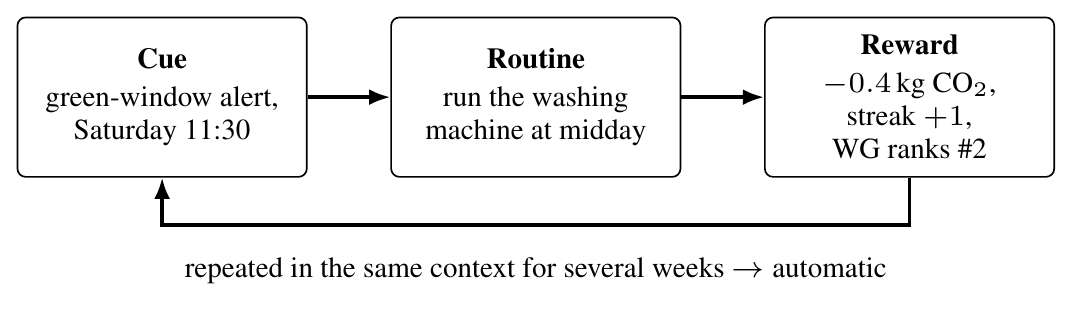
\includegraphics[width=\columnwidth]{figures/habit-loop.png}
\caption{The habit loop on which every screen of the app is based.}
\label{fig:loop}
\end{figure}

Nudging raises ethical questions, and the course brief explicitly asks for ethical AI and transparency. Home Energy Coach therefore uses only opt-in nudges: users choose their own commitments, every recommendation carries a ``why this'' explanation, notifications can be muted per habit, and prompts fade automatically once a habit is established. The WG challenge shows the shared score of the flat, not who did what, to avoid pressure between flatmates. No dark patterns -- artificial scarcity, guilt messages, hidden opt-outs -- are used.

\subsection{Testing and Quality Assurance}
Testing starts as soon as the first components exist in Sprint~3 and covers three levels: \textbf{unit tests} for the R functions (\pkg{testthat}) and the back-end services (\pkg{pytest}), \textbf{integration tests} for the FastAPI--\pkg{plumber} bridge and the SMARD ingestion -- with recorded API responses as fixtures, so that the tests do not depend on the live service -- and \textbf{end-to-end tests} of the main user flows from onboarding through recommendation, commitment and check-in. GitHub Actions runs the test suites on every pull request, and Docker keeps the test environment identical for all members. Sprint~5 adds a pilot: the team members use the app for two weeks, which yields the first real check-in data, usability feedback and the before/after measurements needed for the evaluation in Section~\ref{sec:ml}.

\subsection{Green Software Engineering: the App's Own Footprint}
Evaluating and optimising the application's own greenness is a core grading theme of the course, not an extra. The team follows three steps that correspond to the aspects named in the course brief -- internal baselines, comparison against common practice, algorithmic efficiency and documented design choices -- and draws on the Software Carbon Intensity specification of the Green Software Foundation for the choice of metrics~\cite{gsf-sci}.
\begin{enumerate}
\item \textbf{Baseline (Sprint~4).} The first prototype is measured on the client (Lighthouse~\cite{lighthouse} for the web app, the Xcode Energy Gauge for iOS), on the server (CPU time, memory and network bytes per request from Docker statistics and API metrics) and in R (runtime and memory of every analytics job with \pkg{bench} and \pkg{profvis}). The baseline is documented and targets are set for the following sprints.
\item \textbf{Optimise.} Analytics run as nightly batch jobs instead of per request; SMARD data, the daily green-window forecast and the recommendations are computed once and cached; payloads are kept lean and paginated; notifications are only sent for green windows that match the user's schedule; and algorithmic alternatives for the models in Section~\ref{sec:ml} are compared by runtime and memory as well as by accuracy.
\item \textbf{Prove it.} Every sprint the measurements are repeated, the trend is recorded and shown on the in-app screen ``How green is this app?''. Each design decision and its measured effect is documented in the final report.
\end{enumerate}

\begin{figure*}[!t]
\centering
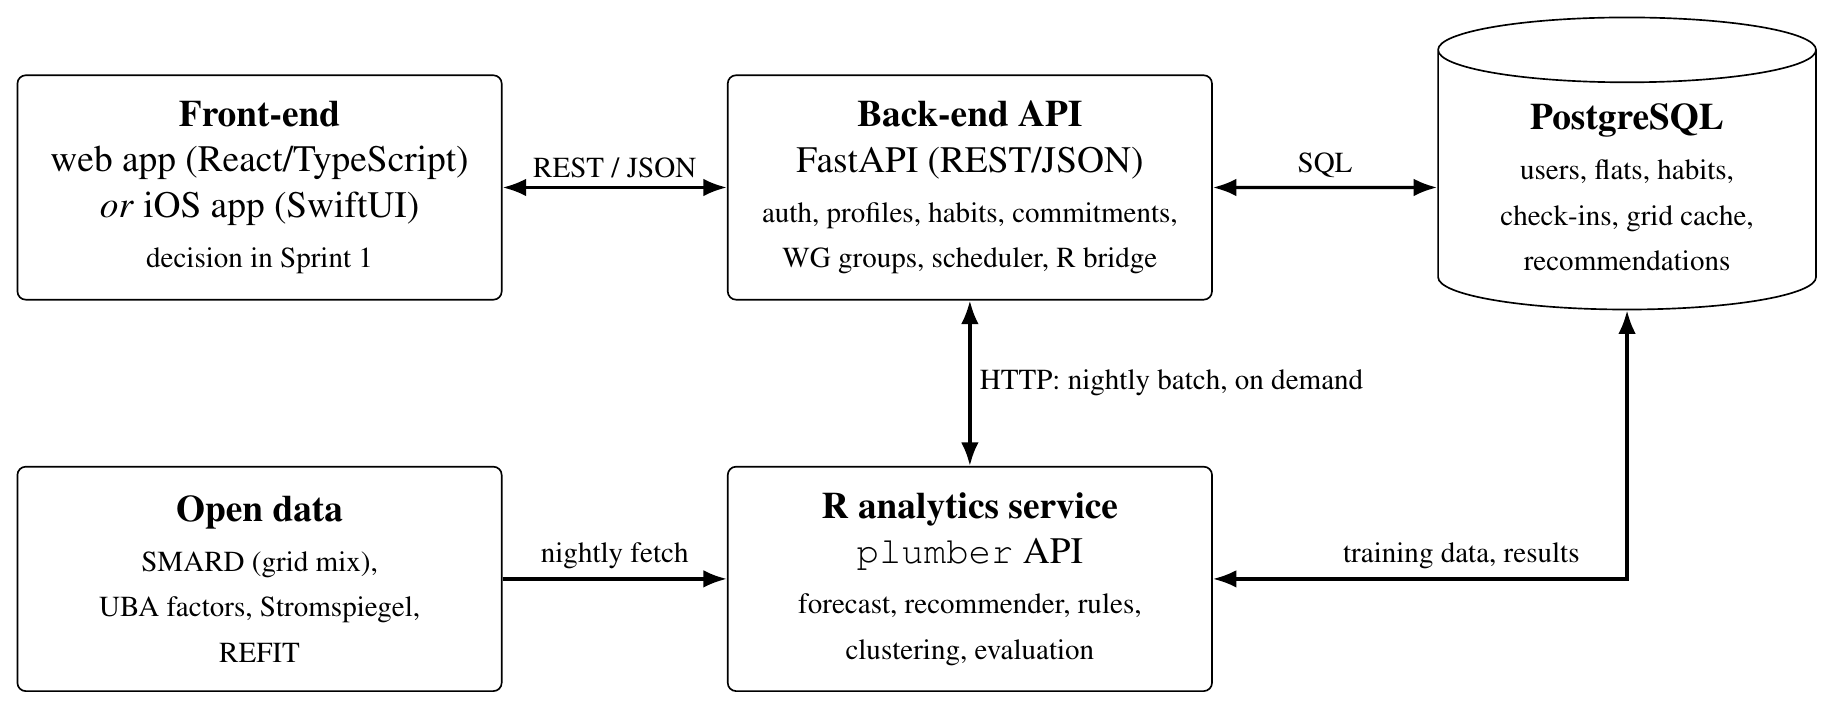
\includegraphics[width=0.92\textwidth]{figures/architecture.png}
\caption{High-level system architecture: a layered client--server system in which R runs isolated in its own analytics service. All components run as Docker containers.}
\label{fig:arch}
\end{figure*}

\section{System Architecture}
The platform uses a \textbf{layered client--server architecture with a separate analytics service} (Fig.~\ref{fig:arch}): a front-end layer, a back-end layer built with FastAPI, an analytics layer in R and a data layer. All communication between components runs over REST endpoints with JSON payloads; the front-end never talks to R directly. This split is deliberate. The course requires R for all analysis tasks, and isolating R in its own service keeps the general-purpose back-end simple, lets the analytics run as scheduled batch jobs -- which is also the most energy-efficient option -- and allows the back-end and the analytics to be developed and tested independently by different team members. The style is easy to justify and document in the architecture deliverable of Sprint~2.

\subsection{Frontend Layer}
\label{sec:frontend}
The choice between a web application (TypeScript with React~\cite{react}, installable as a progressive web app) and a native iOS application (SwiftUI~\cite{swiftui}) is deliberately left open in this proposal and is taken in Sprint~1 against four criteria: the team's existing skills, support for push notifications (native on iOS; web push requires the installed web app), the available energy measurement tooling (Lighthouse versus the Xcode Energy Gauge), and device reach -- a web app runs on every flatmate's phone regardless of platform. The decision is documented in Jira and reflected in the architecture document of Sprint~2. In both cases the front-end contains the eleven screens of Section~\ref{sec:ui} and communicates only with the back-end API, whose contract is defined first so that back-end development does not depend on the client decision.

\subsection{Backend Layer}
Implemented with FastAPI~\cite{fastapi}. Key components:
\begin{itemize}
\item \textbf{API gateway} -- routing, JWT authentication, request validation.
\item \textbf{Domain services} -- user profiles and flats, the habit catalogue, commitments and check-ins, WG groups, agreements and challenges, notifications.
\item \textbf{Scheduler} -- triggers the nightly SMARD fetch, forecast and recommendation refresh in the R service and sends green-window alerts that match each user's schedule.
\item \textbf{R bridge} -- an HTTP client that calls the \pkg{plumber} endpoints; results are stored in PostgreSQL so that the API serves cached results instead of recomputing them per request.
\end{itemize}

\subsection{Analytics Layer}
The R analytics service exposes its functions through \pkg{plumber}~\cite{plumber}: endpoints for the green-hours forecast, recommendations, personas, association rules and the evaluation reports. It runs in batch mode once per night and on demand only for small requests such as a user's personal green window after a schedule change. The service is stateless, reads from PostgreSQL through a read-only database role (\pkg{DBI}/\pkg{RPostgres}) and writes its results to dedicated tables. The packages used for the models are chosen and justified in Section~\ref{sec:ml}.

\subsection{Data Layer}
\begin{itemize}
\item \textbf{PostgreSQL} -- users, flats (WGs) and memberships, the habit catalogue, commitments, check-ins, notifications, the hourly grid-intensity cache, recommendations and the green measurements of the app itself.
\item \textbf{Open data files} -- the UBA, Stromspiegel and REFIT extracts are versioned in the repository as CSV files and loaded by the R service.
\item \textbf{Privacy} -- the system stores minimal personal data (e-mail address and display name), uses pseudonymous IDs in the analytics service and offers export and deletion of all personal data in the app.
\end{itemize}

\subsection{Containerization and Deployment}
The server side is containerized with Docker~\cite{docker} and orchestrated with Docker Compose. Each major component runs as an isolated service:
\begin{itemize}
\item \texttt{frontend} -- Node-based build of the web application served by nginx (for a native iOS app this service is omitted and the app runs on the device).
\item \texttt{backend} -- Python container running FastAPI with Uvicorn.
\item \texttt{r\_service} -- R container exposing the \pkg{plumber} endpoints.
\item \texttt{scheduler} -- triggers the nightly jobs and the notification run.
\item \texttt{postgres} -- persistent relational storage.
\end{itemize}
A single \texttt{docker-compose.yml} at the repository root defines all services, networks and volumes, so that every member and the instructor can start the full stack with one command. GitHub Actions builds the images and runs the tests on every pull request.

\section{Technology Stack}
Table~\ref{tab:stack} summarises the technologies per layer. The stack deliberately mirrors the architecture: one general-purpose language for the API, R for everything analytical, and a relational database as the single source of truth. All tools are free for students, run on macOS, Windows and Linux, and are available as Docker images, so that no member depends on a particular machine.

\begin{table}[!t]
\caption{Technology Stack}
\label{tab:stack}
\centering
\footnotesize
\begin{tabular}{@{}lL{2.9cm}L{2.7cm}@{}}
\toprule
Layer & Technology & Purpose \\
\midrule
Front-end & React (TypeScript) \emph{or} SwiftUI & User interface; decision in Sprint~1 \\
Back-end & Python (FastAPI) & REST API, scheduling, R bridge \\
Analysis & R (\pkg{plumber}) & Forecast, recommender, clustering, evaluation \\
Database & PostgreSQL & Persistent storage, caches \\
Deployment & Docker Compose, GitHub Actions & Containers, CI \\
Design & Figma & Wireframes and mockups \\
Modelling & draw.io / PlantUML & UML diagrams \\
Management & Jira, GitHub & Backlog, Scrum evidence, code \\
\bottomrule
\end{tabular}
\end{table}

\section{User Interfaces}
\label{sec:ui}
Eleven interfaces are planned beyond basic CRUD and authentication, three more than the eight required, so that the scope can be reduced without falling below the requirement:
\begin{enumerate}
\item \textbf{Onboarding energy quiz} -- flat size, flatmates, heating type, appliances and weekly schedule, with an immediate ``similar flats'' comparison.
\item \textbf{Energy dashboard} -- estimated monthly kWh, \COtwo{} and euro per end use, and the progress of the current habits.
\item \textbf{Recommendation feed with ``why this''} -- ranked habits, each with the reason it was chosen for this user.
\item \textbf{Habit commitment and check-in} -- choose a goal, define when and where it happens, log completions, see the streak.
\item \textbf{Green Hours planner} -- today's and tomorrow's grid \COtwo{} curve with the user's personal green windows and reminders.
\item \textbf{Habit library} -- all 22 habits with saving estimates, filterable by type and effort.
\item \textbf{One-time checklist} -- one-off actions with their lifetime saving.
\item \textbf{WG agreement and challenge} -- shared goals and house rules of the flat and the ranking between flats.
\item \textbf{Trends and analytics} -- weekly and monthly development, before/after comparison of adopted habits.
\item \textbf{Privacy and data centre} -- what is stored, export and deletion, notification settings.
\item \textbf{``How green is this app?''} -- the measured footprint of the application itself, sprint by sprint.
\end{enumerate}
Wireframes are developed in Figma in Sprint~2 and refined into mockups in Sprint~4.

\section{Risks and Mitigation}
Table~\ref{tab:risks} lists the main risks identified during topic selection and how the team intends to handle them. The risk register is kept in Jira and reviewed in every Sprint Retrospective.

\begin{table}[!t]
\caption{Risks and Mitigation}
\label{tab:risks}
\centering
\footnotesize
\begin{tabular}{@{}L{3.3cm}L{5cm}@{}}
\toprule
Risk & Mitigation \\
\midrule
No real users to train models on & Synthetic users from Stromspiegel, UBA and REFIT; survey in Sprint~2; pilot with the team in Sprint~5 \\
Users cannot measure their own kWh & Estimate from the profile and public statistics; optional meter readings \\
SMARD API changes or downtime & Nightly caching; fallback to the stored dataset; ingestion isolated in one R module \\
R skills uneven across the team & Two R owners; shared R scripts; pair-programming sessions \\
Nudges feel manipulative or annoying & User-chosen commitments, mute option, ``why this'' on every tip, prompts fade once a habit is formed \\
Front-end decision delays development & Decision in Sprint~1 against fixed criteria; API contract defined first so the back-end is independent of the client \\
Scope too large for one semester & Eight screens required, eleven planned; the additional screens are the first candidates to be descoped \\
\bottomrule
\end{tabular}
\end{table}

\section{Deliverables}
\begin{enumerate}
\item Personas, scenarios and user stories
\item Wireframes and mockups (Figma)
\item System architecture document with justification of the architectural style
\item UML models: use case, class, activity and sequence diagrams
\item Working application with back-end, front-end and R analytics service, containerized with Docker
\item Green software evaluation: baseline, optimisations and measured trend of the app's own footprint
\item Jira project with Scrum evidence, artifacts and team contract, accessible to the instructor
\item User documentation and final project report
\end{enumerate}

\begin{thebibliography}{00}
\bibitem{rcore} R Core Team, \emph{R: A Language and Environment for Statistical Computing}, R Foundation for Statistical Computing, Vienna, Austria, 2025. [Online]. Available: \url{https://www.R-project.org/}
\bibitem{scrumguide} K. Schwaber and J. Sutherland, ``The Scrum Guide,'' 2020. [Online]. Available: \url{https://scrumguides.org/}
\bibitem{smard} Bundesnetzagentur, ``SMARD -- Strommarktdaten: Electricity market data for Germany,'' data download and API. [Online]. Available: \url{https://www.smard.de/}
\bibitem{uba-strommix} Umweltbundesamt, ``Entwicklung der spezifischen Treibhausgas-Emissionen des deutschen Strommix in den Jahren 1990--2025,'' Dessau-Ro\ss lau, Mar. 2026. [Online]. Available: \url{https://www.umweltbundesamt.de/themen/co2-emissionen-pro-kilowattstunde-strom-2025-nur}
\bibitem{stromspiegel} co2online gGmbH, ``Stromspiegel 2025: Deutsche Haushalte verschwenden j\"ahrlich 12 Milliarden Euro f\"ur Strom,'' press release, Berlin, May 2025. [Online]. Available: \url{https://www.stromspiegel.de/}
\bibitem{uba-haushalte} Umweltbundesamt, ``Energieverbrauch privater Haushalte,'' data and Excel downloads, 2026. [Online]. Available: \url{https://www.umweltbundesamt.de/daten/private-haushalte-konsum/wohnen/energieverbrauch-privater-haushalte}
\bibitem{refit} D. Murray, L. Stankovic, and V. Stankovic, ``An electrical load measurements dataset of United Kingdom households from a two-year longitudinal study,'' \emph{Scientific Data}, vol.~4, art.~160122, 2017, doi: 10.1038/sdata.2016.122.
\bibitem{bunddev} \emph{bunddev: R Client for the bund.dev Public APIs}, R package, CRAN, 2026. [Online]. Available: \url{https://cran.r-project.org/package=bunddev}
\bibitem{fogg2009} B. J. Fogg, ``A behavior model for persuasive design,'' in \emph{Proc. 4th Int. Conf. Persuasive Technology (Persuasive '09)}, Claremont, CA, USA, 2009, art.~40.
\bibitem{gollwitzer1999} P. M. Gollwitzer, ``Implementation intentions: Strong effects of simple plans,'' \emph{American Psychologist}, vol.~54, no.~7, pp.~493--503, 1999.
\bibitem{lally2010} P. Lally, C. H. M. van Jaarsveld, H. W. W. Potts, and J. Wardle, ``How are habits formed: Modelling habit formation in the real world,'' \emph{European Journal of Social Psychology}, vol.~40, no.~6, pp.~998--1009, 2010.
\bibitem{gsf-sci} Green Software Foundation, ``Software Carbon Intensity (SCI) Specification,'' ISO/IEC 21031:2024. [Online]. Available: \url{https://sci.greensoftware.foundation/}
\bibitem{plumber} B. Schloerke and J. Allen, \emph{plumber: An API Generator for R}, R package. [Online]. Available: \url{https://www.rplumber.io/}
\bibitem{fastapi} S. Ram\'irez, ``FastAPI: Modern, fast web framework for building APIs with Python.'' [Online]. Available: \url{https://fastapi.tiangolo.com/}
\bibitem{react} Meta Platforms, Inc., ``React -- The library for web and native user interfaces.'' [Online]. Available: \url{https://react.dev/}
\bibitem{swiftui} Apple Inc., ``SwiftUI.'' [Online]. Available: \url{https://developer.apple.com/xcode/swiftui/}
\bibitem{docker} Docker, Inc., ``Docker: Accelerated container application development.'' [Online]. Available: \url{https://www.docker.com/}
\bibitem{lighthouse} Google LLC, ``Lighthouse.'' [Online]. Available: \url{https://developer.chrome.com/docs/lighthouse/}
\end{thebibliography}

\end{document}
